%****************************************************************
% Chapter X
%****************************************************************
\chapter{Performance}
\label{chapter-performance}

What is great about the Android runtime is that most of the stress of memory reclamation is done for developers. The system will track what developers are doing and when it sees that an object is not needed anymore, it will free it on their behalf. However, this does not exclude performance problems from happening here. When the amount of memory have allocated reaches an upper limit, a Garbage Collection (GC) event will be kicked off to free any resources that might not be needed any longer, freeing up space for future allocations. 

Anytime the frame drips about the $16$ms barrier, and the users are going to start to notice. Therefore, any code that forces allocated memory to spike above this threshold can cause problems. For instance, memory can become tighter, if the developer is allocating and freeing a large number of objects in a short period of time, the temporary objects again kicking off GC event. 

\begin{figure}[H]
\caption{16ms per frame}
\label{fig:16ms-per-frame}
\centering
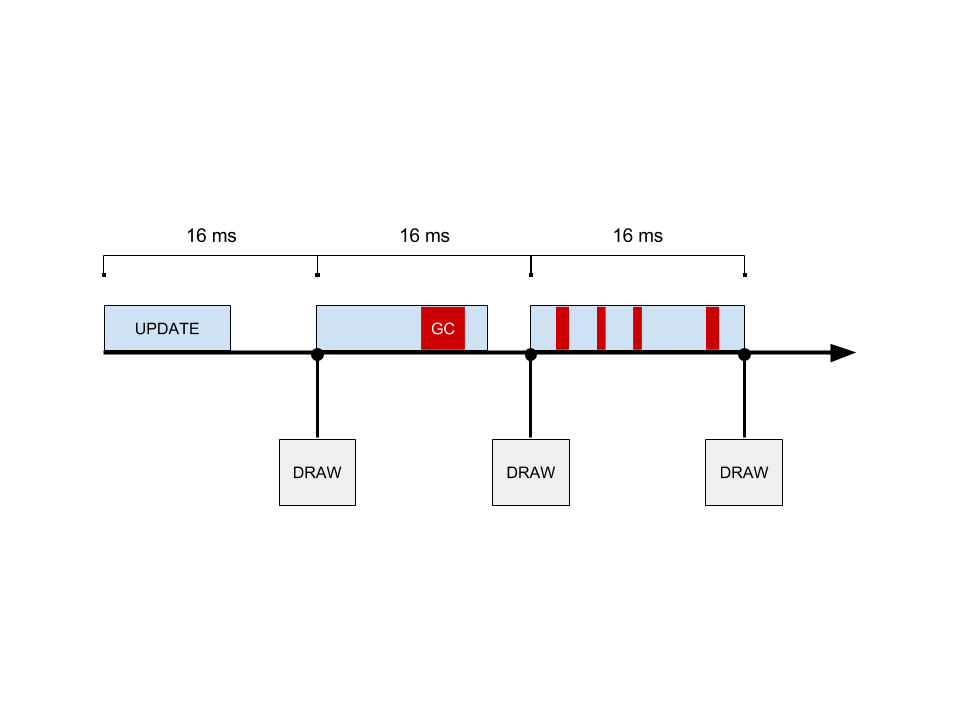
\includegraphics[width=\textwidth, keepaspectratio]{Figures/16ms-per-frame.png}
\decoRule
\end{figure}

Therefore, a performance testing is important for avoiding nasty GC events. Each GC event that developer can avoid, the application has more time per frame to do interesting things. In order to find out where in the code objects are being created but not released, created and not used, or created new when the developer could have been reusing them from existing objects. Android Studio provides a series of performance testing tools, such as Memory Monitor, Allocation Tracker, Heap Viewer, and the Systrace (it is an Android system trace tool helps developers analyze how the execution of the application fits into the many running systems on an Android device \cite{google.systrace.2016}). According to the runtime, the performance analysis is divided into two parts: acyclic process and cyclic process (performance data came from Android phone $Nexus\;6P$ \footcite{CPU: 2.0GHz octa-core, 64-bit ARM Cortex-A57 & ARM Cortex-A53, 8 cores; GPU: Adreno 430}).

%****************************************************************
\section{Initialization}

In order to avoid UI being block, initialization processes in the application are handled in the asynchronous thread. In this section, I present the performance of geometric vertices' generation for \code{Placemark} (Icosphere) and \code{Earth} (UV sphere) which only executes one time (or not) when needed. The geometric data from Icosphere generation will be cached once it has been created. This is useful to avoid duplicate creations for same geometric vertices.

%****************************************************************
\subsection{Icosphere Generator}

Based on the varying roundness of the Icosphere, it could evolve into spheres have different vertex count (). In general, level $3$ Icosphere is enough for illustrating a sphere, and in the application the \code{Placemark} is created on level $1$ Icosphere. See the performance testing result from $40$ data sets each (Table \ref{tab:icosphere-generation-performance}), even for a particular reason that requires a level $5$ Icosphere, less than $300$ms is acceptable as an one time asynchronous task.

\begin{table}[H]
	\caption{Icosphere generation performance}
	\label{tab:icosphere-generation-performance}
	\centering
	\begin{tabular}{l l l l}
		\toprule
		\tabhead{Recursion Level} & \tabhead{Vertex Count} & \tabhead{Mean Value (ms)} & \tabhead{Stand Deviation (ms)}\\
		\midrule
		0 & 12 & 0.049 & 0.014 \\
		1 & 42 & 0.257 & 0.490 \\
		2 & 162 & 0.722 & 0.250 \\
		3 & 642 & 3.296 & 0.707 \\
		4 & 2562 & 19.988 & 3.050 \\
		5 & 10242 & 148.927 & 18.422 \\
		\bottomrule
	\end{tabular}
\end{table}

\begin{figure}[H]
	\caption{Icosphere performance sets}
	\label{fig:icosphere-performance-sets}
	\centering
	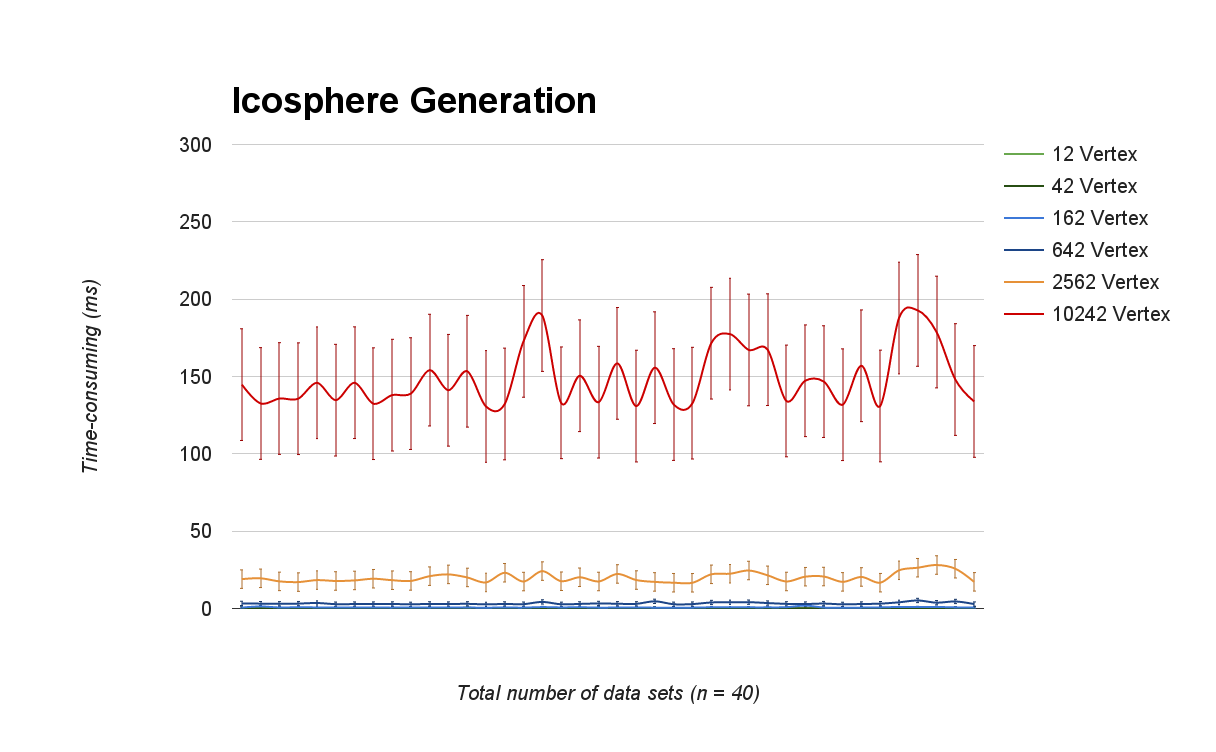
\includegraphics[width=0.9\textwidth, keepaspectratio]{Figures/icosphere-performance-sets.png}
	\decoRule
\end{figure}

\begin{figure}[H]
	\caption{Icosphere performance loglog}
	\label{fig:icosphere-performance-loglog}
	\centering
	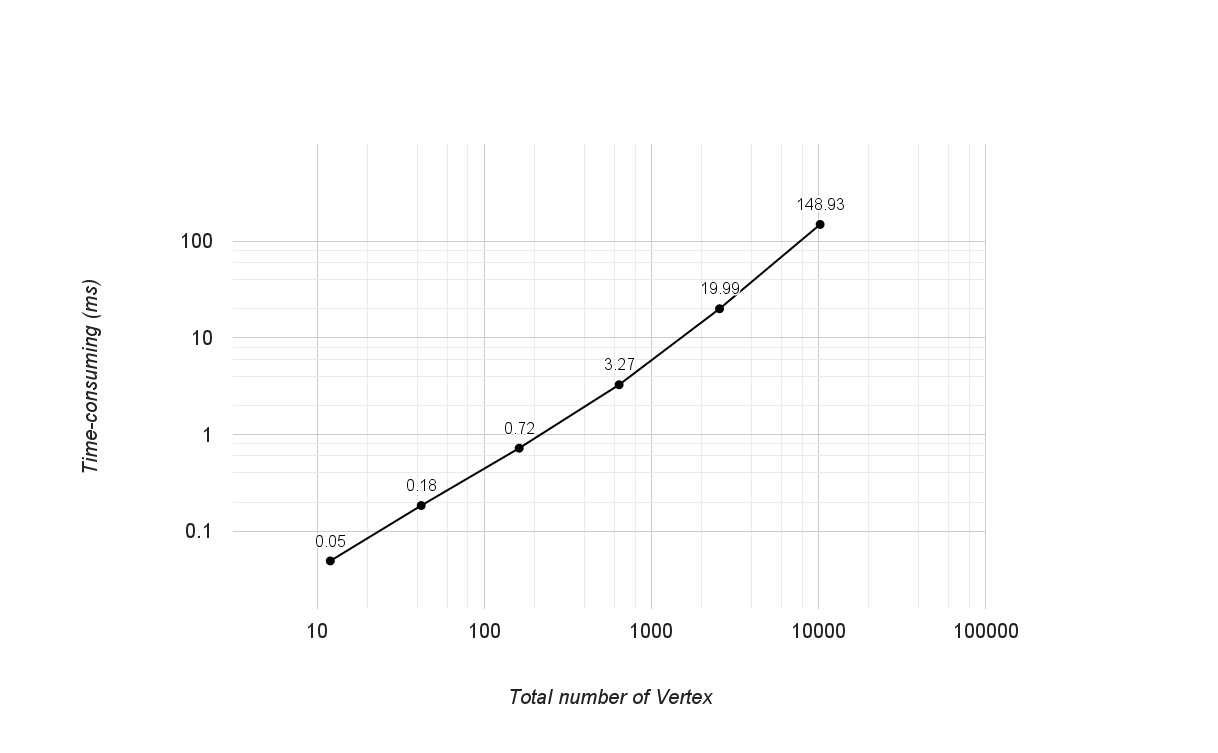
\includegraphics[width=0.9\textwidth, keepaspectratio]{Figures/icosphere-performance-loglog.png}
	\decoRule
\end{figure}

%****************************************************************
\subsection{UV Sphere Generator}

The roundness of a UV sphere depends on the partition level on both horizontal (ring) and vertical (segment) which denotes the axes of the 2D texture. The Earth is casually implemented as a "$180:180$" UV sphere in the application. Table \ref{tab:uv-sphere-generation-performance} shows the testing result from $40$ data sets each.

\begin{table}[H]
	\caption{UV sphere generation performance}
	\label{tab:uv-sphere-generation-performance}
	\centering
	\begin{tabular}{l l l l}
		\toprule
		\tabhead{Partition Level} & \tabhead{Vertex Count} & \tabhead{Mean Value (ms)} & \tabhead{Stand Deviation (ms)}\\
		\midrule
		5:5 & 25 & 0.100 & 0.033 \\
		10:10 & 100 & 0.201 & 0.072 \\
		20:20 & 400 & 0.322 & 0.100 \\
		40:40 & 1600 & 2.098 & 0.699 \\
		80:80 & 6400 & 5.431 & 1.153 \\
		160:160 & 25600 & 17.050 & 2.084 \\
		\bottomrule
	\end{tabular}
\end{table}

\begin{figure}[H]
	\caption{UV sphere performance sets}
	\label{fig:uv-sphere-performance-sets}
	\centering
	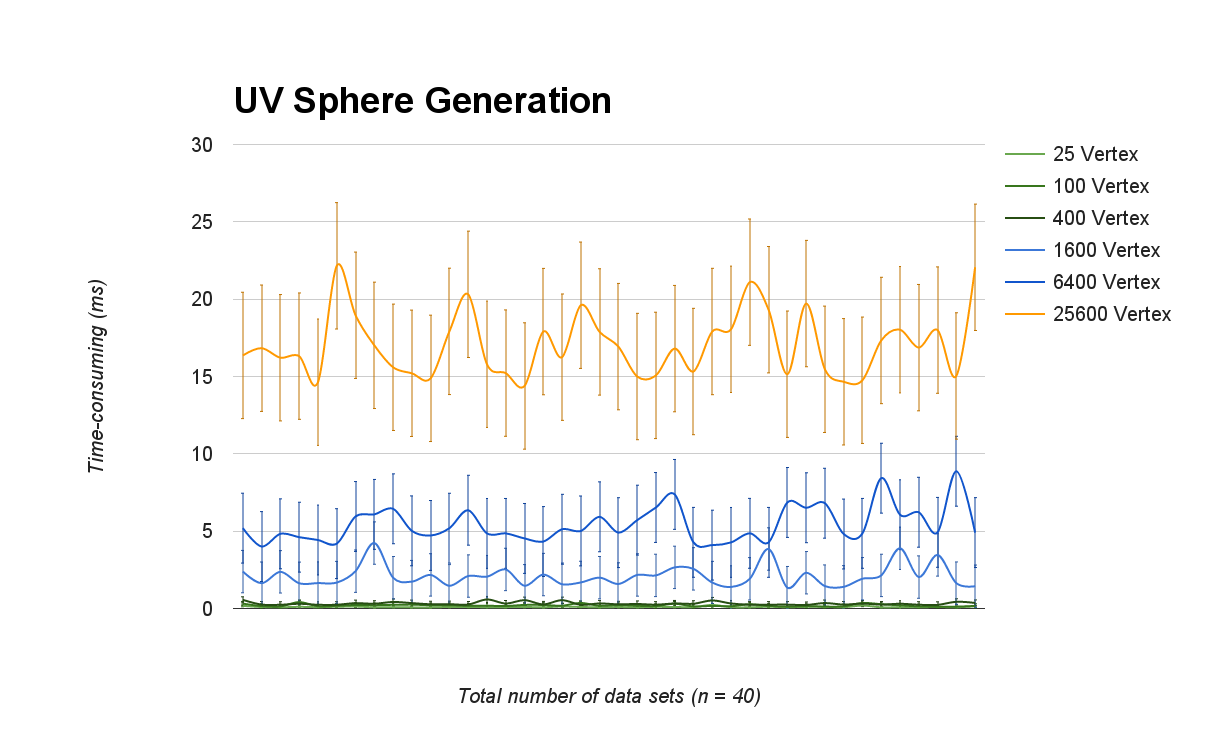
\includegraphics[width=0.9\textwidth, keepaspectratio]{Figures/uv-sphere-performance-sets.png}
	\decoRule
\end{figure}

\begin{figure}[H]
	\caption{UV sphere performance loglog}
	\label{fig:uv-sphere-performance-loglog}
	\centering
	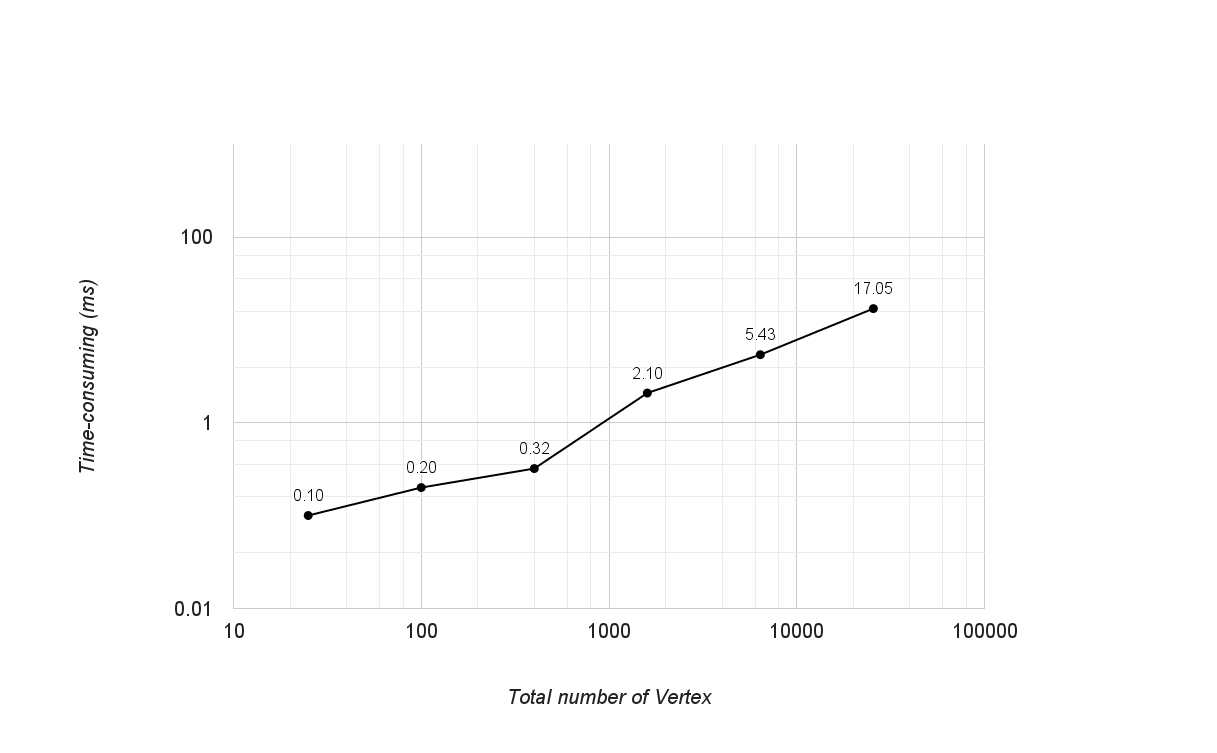
\includegraphics[width=0.9\textwidth, keepaspectratio]{Figures/uv-sphere-performance-loglog.png}
	\decoRule
\end{figure}

By comparison, to rounding Icosphere by Java program, UV sphere generation has better performance when the application requires a very smooth, detailed surface. In the program, UV sphere vertex is not cached after created. Because it does not make much sense to cache such data for a "$n:m$" UV sphere, where the $n$ (rings) and $m$ (segments) could be any positive number. On the other side, Icosphere is created by a given level which defines the vertices.

\begin{figure}[H]
	\caption{Sphere generation}
	\label{fig:icosphere-and-uv-sphere}
	\centering
	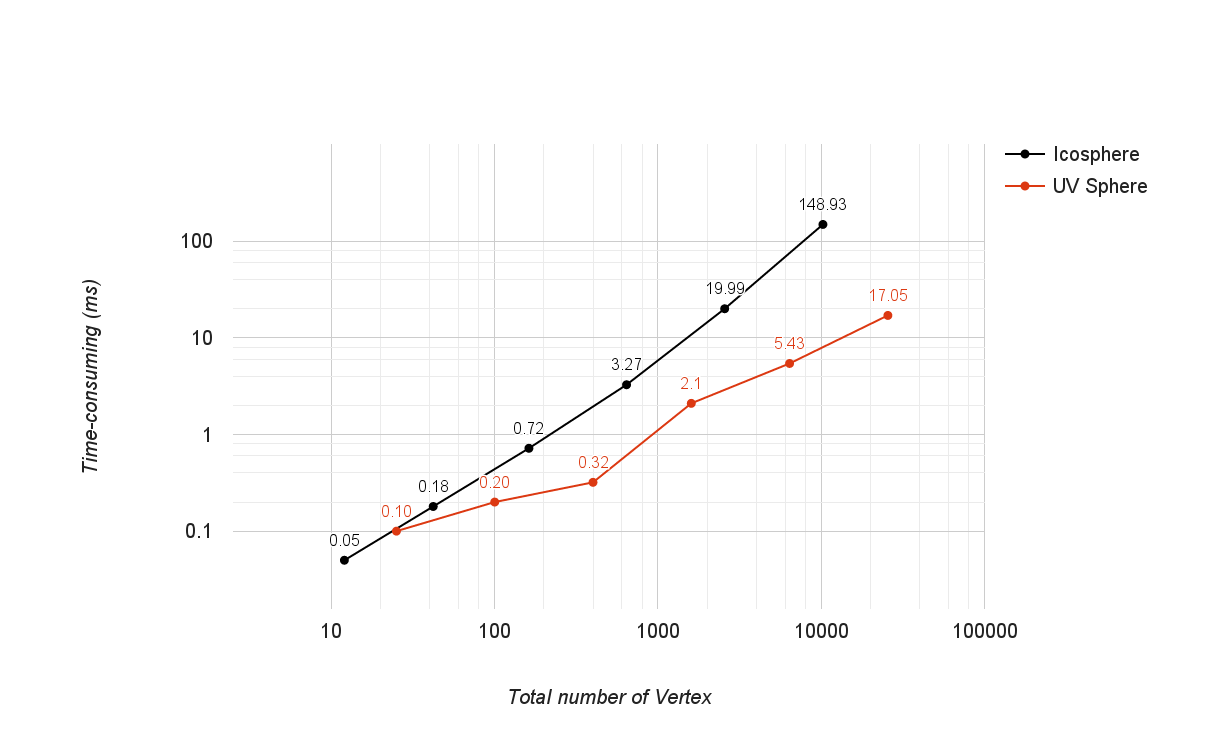
\includegraphics[width=0.9\textwidth, keepaspectratio]{Figures/icosphere-and-uv-sphere.png}
	\decoRule
\end{figure}

%****************************************************************
\subsection{Geographic Data Initialization}

Table \ref{tab:geographic-data-performance} is the performance ($10$ data sets) of initializing geographic data, including parsing KML files, transformation coordinate system from LLA to ECEF, space partition, etc. The number of time-consuming has linear increase with the size of \code{Placemark}, see following testing result from $10$ data sets each. There are reasons I did not separate this processes into many. First, the space partition and KML parsing process will be slightly changed on certain scenarios. They are dependent on how crowded the coordinates are. For instance, if $8$ \code{Placemark} locate in the same place or small area which requires multiple times space-division (limitation of how many models can be contained in one space cell). However, if the $8$ coordinates happen to separately locate at different corners area which only requires one time space division ($1$ space cell divides into $8$ space cells). Moreover, it depends on how many KML links (URL points to another KML file, and another again), are they have force update from server property. I have a limited time on creating such proper data for testing.

\begin{table}[H]
	\caption{Geographic data performance}
	\label{tab:geographic-data-performance}
	\centering
	\begin{tabular}{l l l}
		\toprule
		\tabhead{Placemark Count} & \tabhead{Mean Value (ms)} & \tabhead{Stand Deviation (ms)}\\
		\midrule
		10 & 29.965 & 3.235 \\
		20 & 53.441 & 3.551 \\
		40 & 119.092 & 5.128 \\
		80 & 229.839 & 13.266 \\
		160 & 446.349 & 25.377 \\
		320 & 882.641 & 32.351 \\
		\bottomrule
	\end{tabular}
\end{table}

\begin{figure}[H]
	\caption{Geographic data performance sets}
	\label{fig:geographic-data-performance-sets}
	\centering
	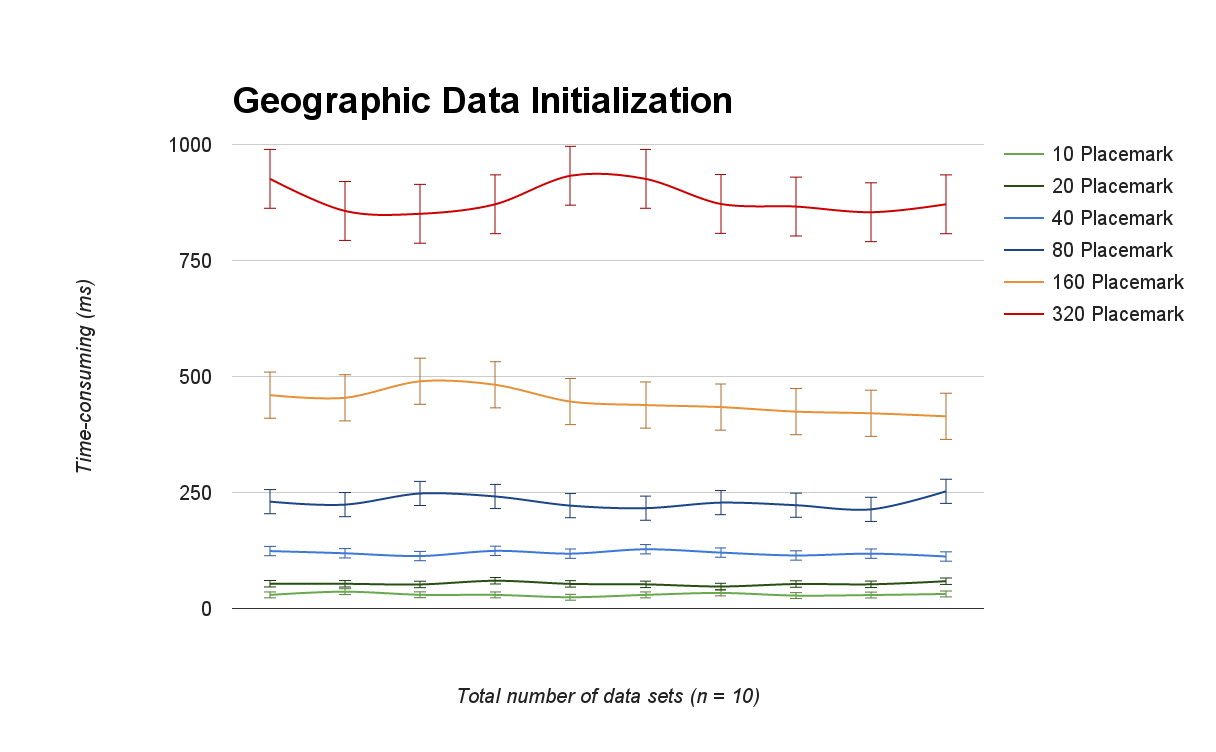
\includegraphics[width=0.9\textwidth, keepaspectratio]{Figures/geographic-data-performance-sets.png}
	\decoRule
\end{figure}

\begin{figure}[H]
	\caption{Geographic data performance loglog}
	\label{fig:geographic-data-performance-loglog}
	\centering
	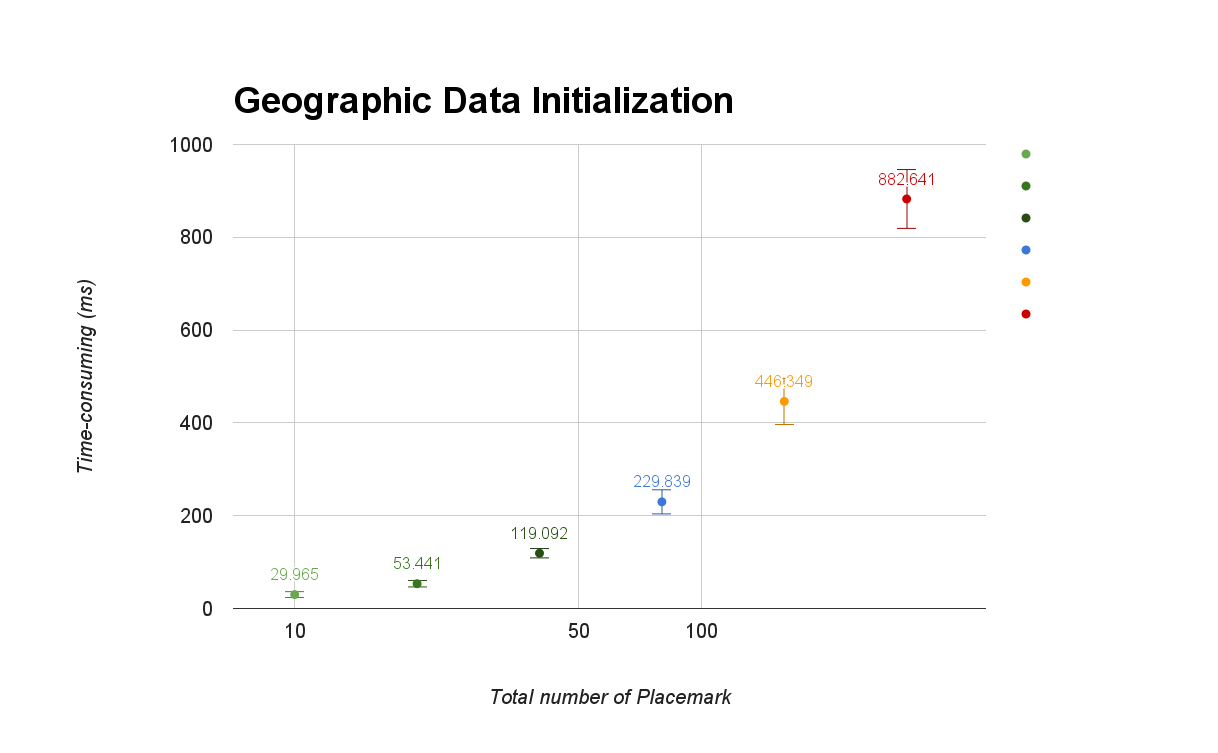
\includegraphics[width=0.9\textwidth, keepaspectratio]{Figures/geographic-data-performance-loglog.png}
	\decoRule
\end{figure}

%****************************************************************
\section{Runtime}

Tasks that require continually repeated during the render loop is the factors influencing the runtime performance. They are ray-model intersection detection, update models and draw models. In this section, I present memory leak analysis during the loop, as well as the tasks that closely related to performance.
 
\begin{figure}[H]
	\caption{Runtime task}
	\label{fig:runtime-task}
	\centering
	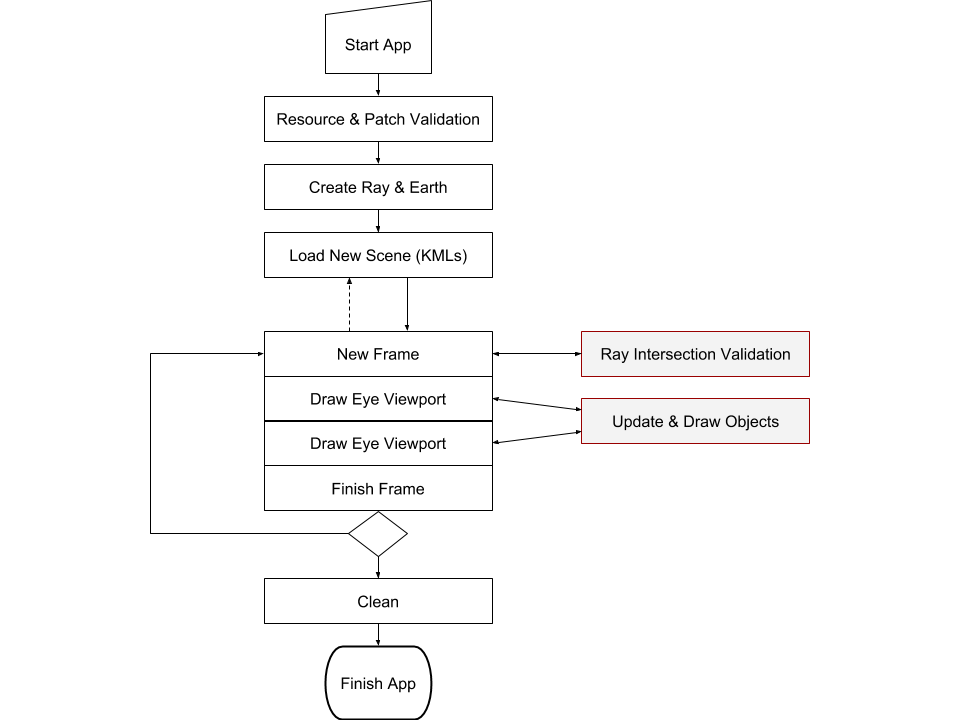
\includegraphics[width=\textwidth, keepaspectratio]{Figures/runtime-task.png}
	\decoRule
\end{figure}


%****************************************************************
\subsection{Memory Leak}

I am using Memory Monitor to evaluate memory leak. As the application allocates and free memory, we will see the allocative amount fluctuate in the graph at the same time. Any time the allocated memory drops by a significant amount, that is a signal that GC event has occurred (see \ref{fig:memory-monitor}). These GC events are not generally a noticeable performance problem. However, lots of them occurring over and over and over again in a short period of time can lead to performance issues. Additionally, it more or less created memory leaks, which are objects which the application is no longer using, but the garbage collector fails to recognize them as unused.

\begin{figure}[H]
	\caption[Memory monitor]{Memory Monitor \cite{google.memory-monitor.2015}}
	\label{fig:memory-monitor}
	\centering
	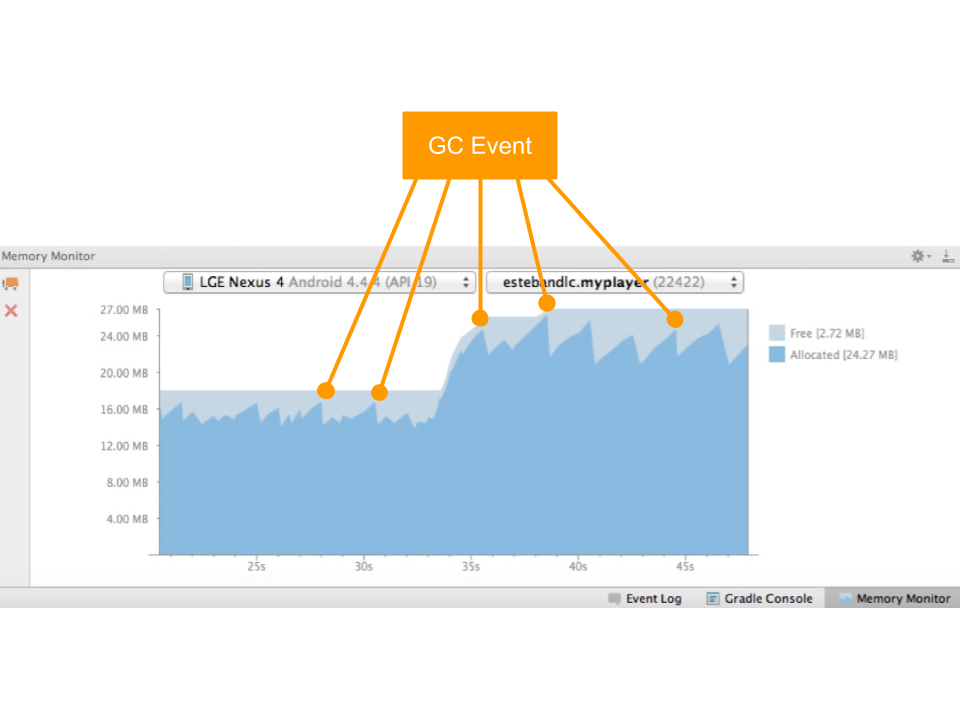
\includegraphics[width=\textwidth, keepaspectratio]{Figures/memory-monitor.png}
	\decoRule
\end{figure}

In a world where the application is not doing much of anything, there will be a flat memory allocation graph. This is an ideal scenario from a performance perspective. The more time is spending doing GC, the less time for the application to do other stuff. Fortunately, with a careful in dealing with objects, I got a quite flat runtime memory allocation \ref{fig:memory-performance}.

\begin{figure}[H]
	\caption{Memory performance}
	\label{fig:memory-performance}
	\centering
	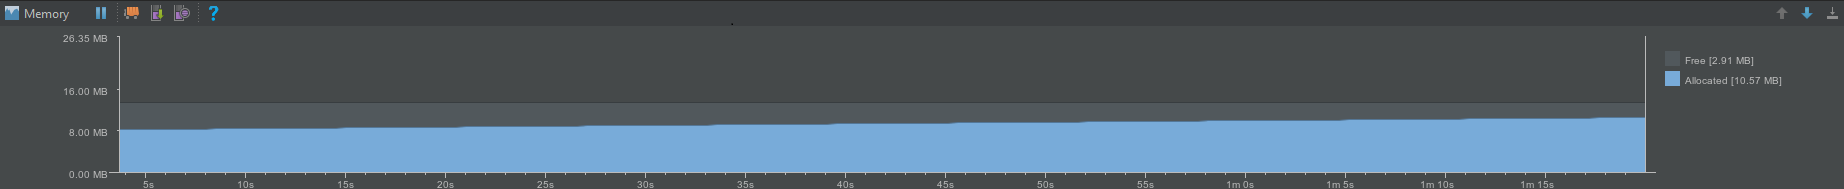
\includegraphics[width=\textwidth, keepaspectratio]{Figures/memory-performance.png}
	\decoRule
\end{figure}

%****************************************************************
\subsection{Placemarks Intersection}
\label{section:placemarks-intersection}

In order to avoid doing ray intersection test on all \code{Placemark} per frame, I implemented octree based space partition to ignore unnecessary detections. There was a significant performance improvement, see performance comparison on Chart \ref{fig:placemark-intersection-performance}. Also as we can from Figure \ref{fig:placemark-intersection-performance-before} and \ref{fig:placemark-intersection-performance-after}, after the optimization, the number of \code{Placemark} is no long relevant. It takes less than $1$ms for hundreds \code{Placemark}.

\begin{figure}[H]
	\caption{Placemark intersection performance - Before}
	\label{fig:placemark-intersection-performance-before}
	\centering
	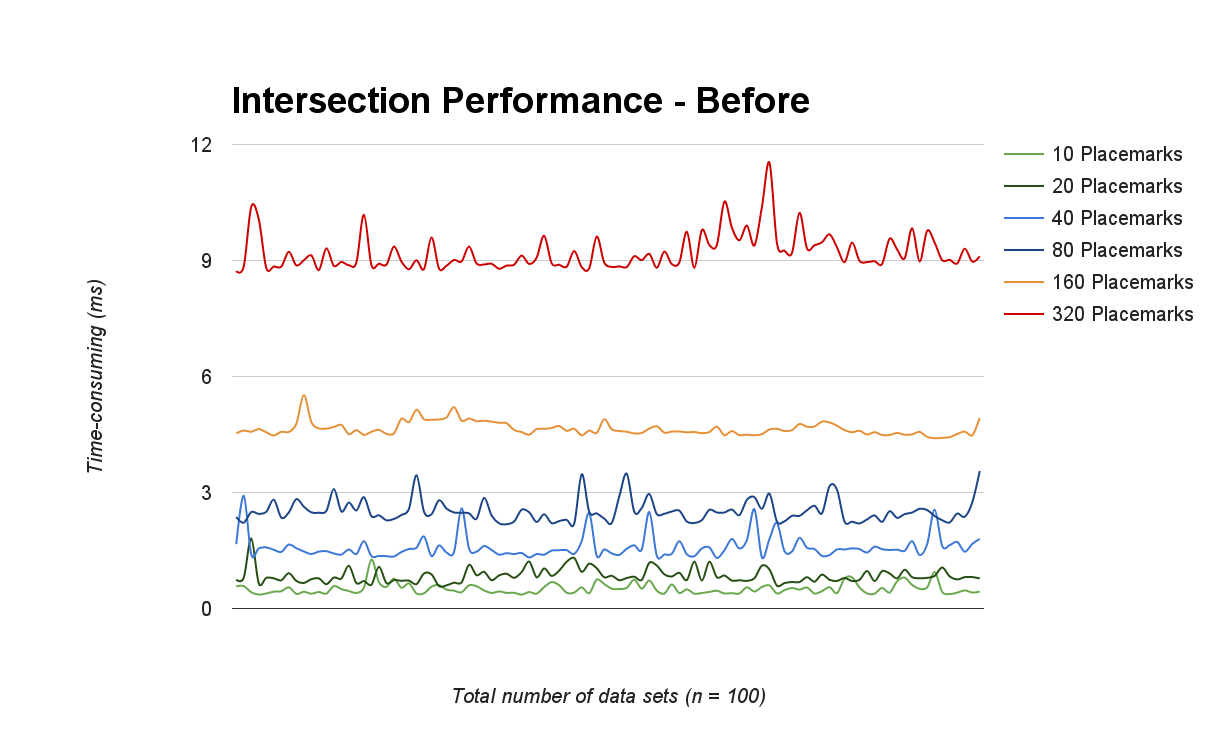
\includegraphics[width=0.9\textwidth, keepaspectratio]{Figures/placemark-intersection-performance-before.png}
	\decoRule
\end{figure}

\begin{figure}[H]
	\caption{Placemark intersection performance - After}
	\label{fig:placemark-intersection-performance-after}
	\centering
	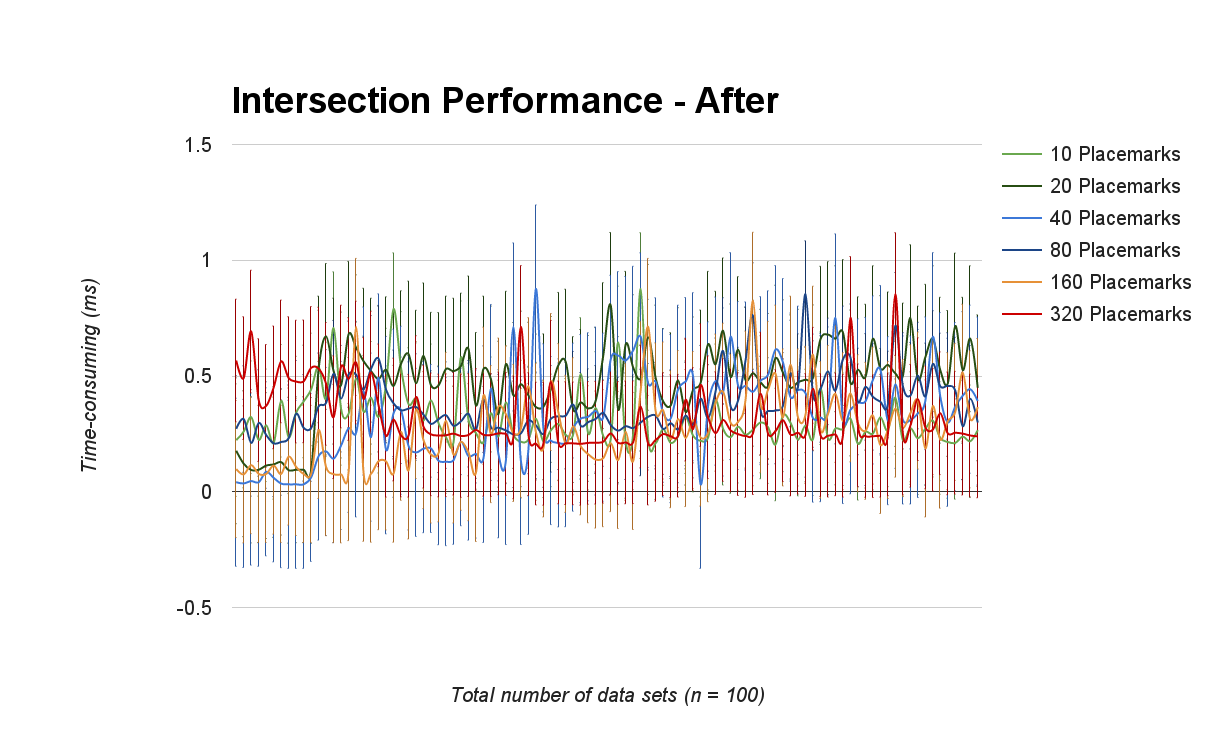
\includegraphics[width=0.9\textwidth, keepaspectratio]{Figures/placemark-intersection-performance-after.png}
	\decoRule
\end{figure}

\begin{figure}[H]
	\caption{Placemark intersection performance}
	\label{fig:placemark-intersection-performance}
	\centering
	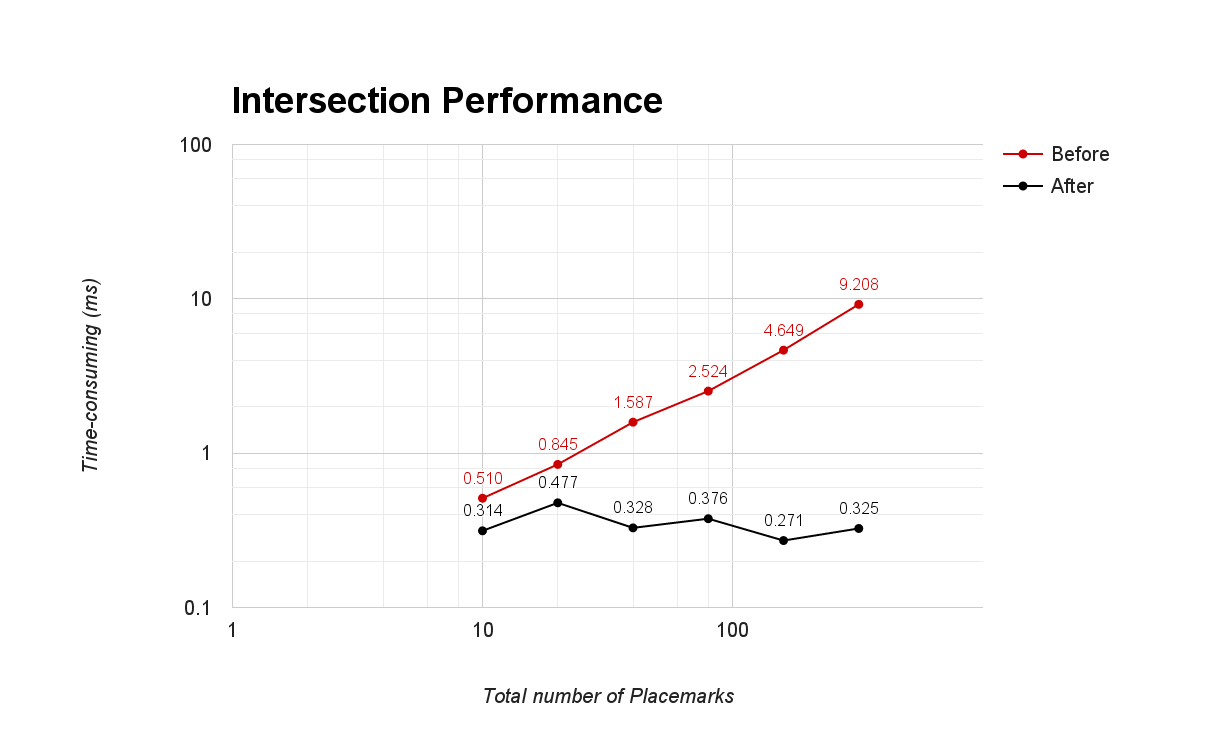
\includegraphics[width=0.9\textwidth, keepaspectratio]{Figures/placemark-intersection-performance.png}
	\decoRule
\end{figure}

%****************************************************************
\subsection{Placemarks Update}
\label{section:placemarks-update}

There was an improvement on model frame update. From doing everything to only doing necessary update. As expected, it ensures a better performance and saves the time for doing other interesting things in the frame. As we can see from following charts, not only it has minimal effect on the number of models, but also performance is reduced under $5$ms.
 
\begin{figure}[H]
	\caption{Placemark update performance - Before}
	\label{fig:placemark-update-performance-before}
	\centering
	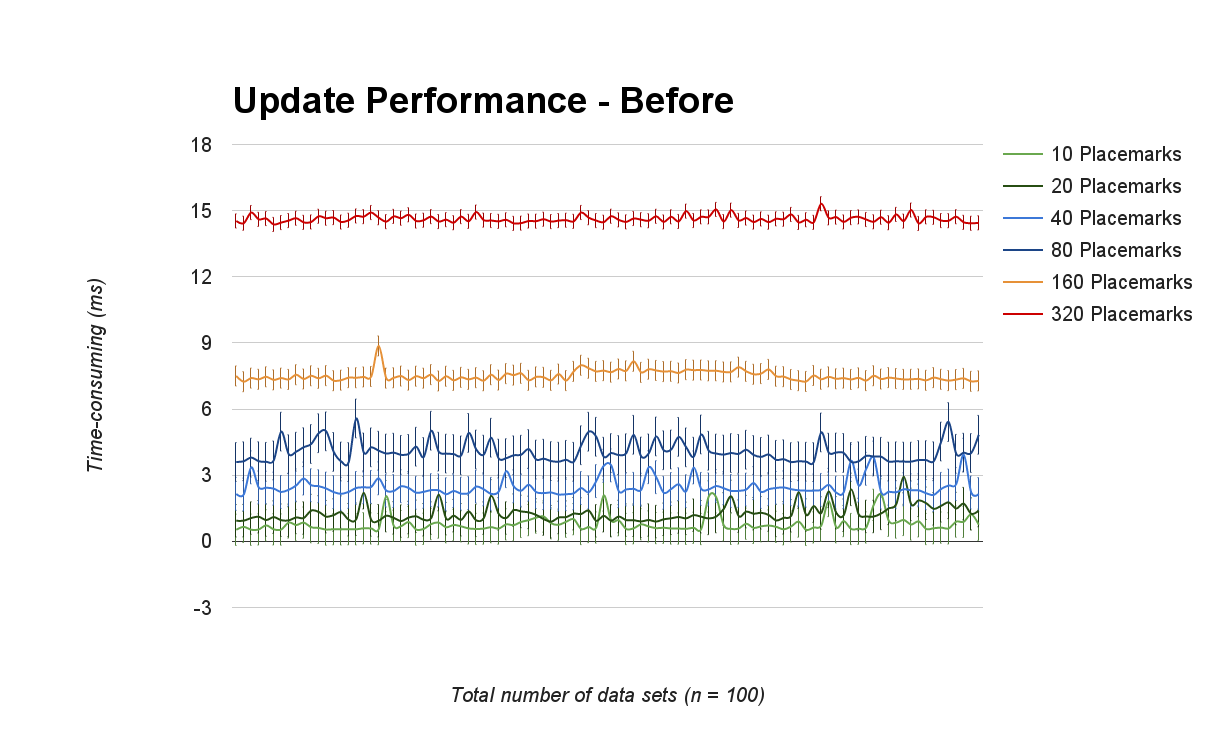
\includegraphics[width=0.9\textwidth, keepaspectratio]{Figures/placemark-update-performance-before.png}
	\decoRule
\end{figure}

\begin{figure}[H]
	\caption{Placemark update performance - After}
	\label{fig:placemark-update-performance-after}
	\centering
	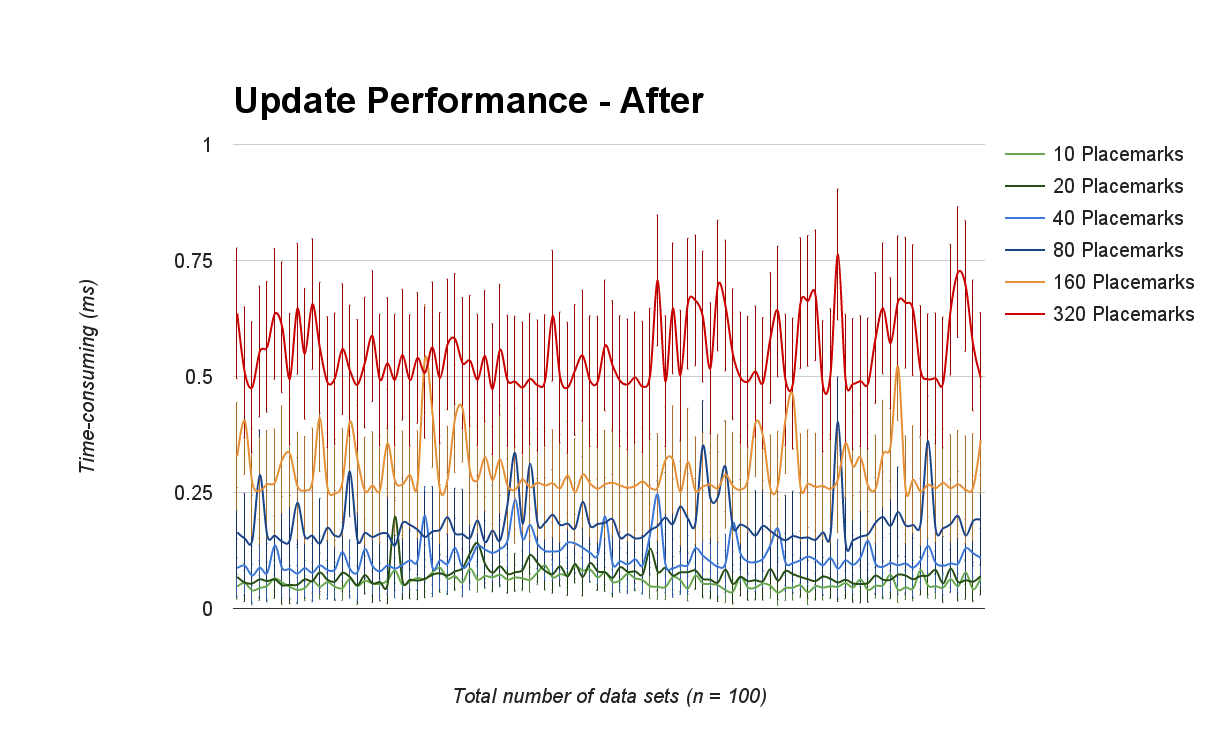
\includegraphics[width=0.9\textwidth, keepaspectratio]{Figures/placemark-update-performance-after.png}
	\decoRule
\end{figure}

\begin{figure}[H]
	\caption{Placemark update performance}
	\label{fig:placemark-update-performance}
	\centering
	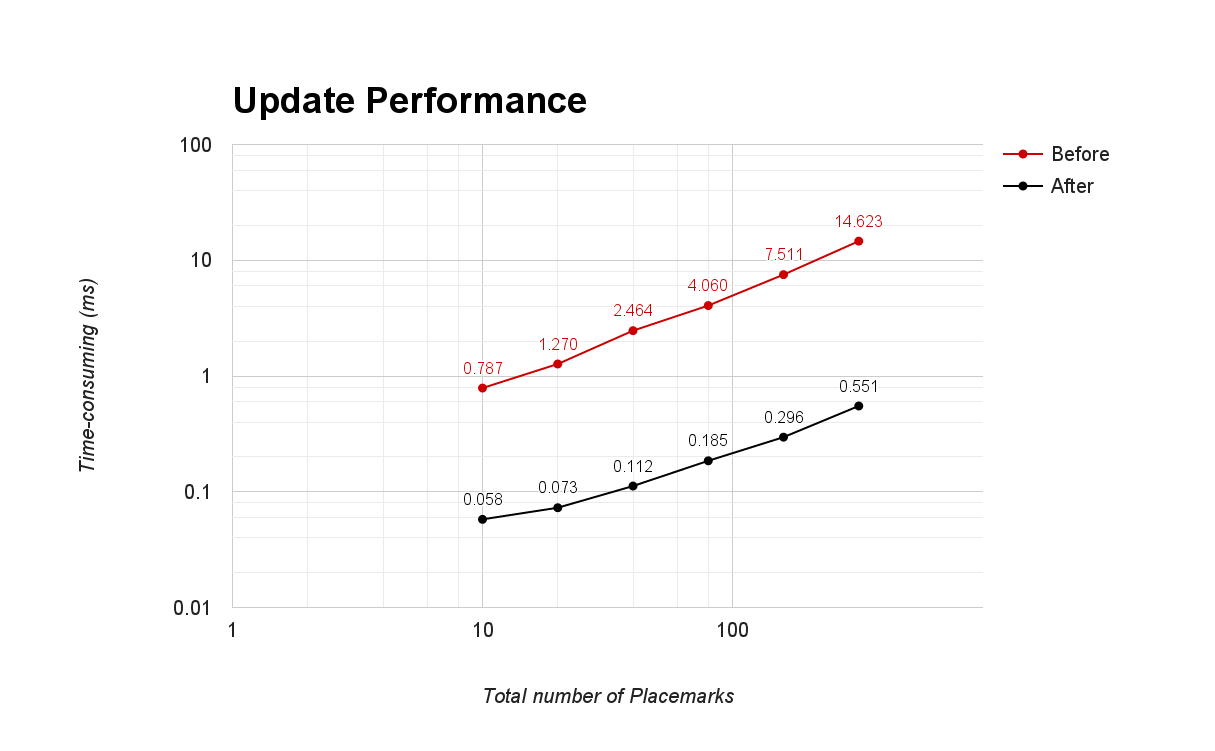
\includegraphics[width=0.9\textwidth, keepaspectratio]{Figures/placemark-update-performance.png}
	\decoRule
\end{figure}

There are mainly $6$ calculations may happens during the frame:

\begin{table}[H]
	\caption{OpenGL compute scope}
	\label{tab:opengl-compute-scope}
	\centering
	\begin{tabular}{l l l l}
		\toprule
		\tabhead{What} & \tabhead{How} & \tabhead{Scope}\\
		\midrule
		Model Matrix & translationM * scaleM * rotationM * identityM(1) & Object specific\\
		Camera Matrix & lookAt(positionV, lookAtV, upV) & Worldwide\\
		View Matrix & eye.viewM * cameraM & Eye specific\\
		Perspective Matrix & eye.perspective(zNear, zFar) & Eye specific\\
		ModelView Matrix & viewM * modelM & Object specific\\
		Projection Matrix & perspectiveM * modelViewM & Object specific\\
		Vertex' & projectionM * vertex & Vertex specific\\
		\bottomrule
	\end{tabular}
\end{table}

Before the improvement, based on the \code{viewM} and \code{perspectiveM} from each eye, computing the \code{modelM}, \code{modelViewM} and \code{projectionM} in CPU for each object per frame. Then pass the \code{modelViewM} and \code{projectionM} to GPU for further calculation, such as lighting and position (\code{Vertex'}). It may create huge performance risk due to a large amount of computation can be omitted. There is no need to re-calculate an object's \code{modelM} per frame if the object has the same position, scale, and rotation. Therefore, application only re-calculate the \code{modelM} for necessary objects, and objects pass the \code{modelM}, \code{viewM} and \code{perspectiveM} to GPU for the rest of calculation. Although it increases the workload in GPU as well as duplicated calculation, but performance is improved in compare with before.

\begin{table}[H]
	\caption{OpenGL compute optimization}
	\label{tab:opengl-compute-optimization}
	\centering
	\begin{tabular}{l l l l}
		\toprule
		\tabhead{What} & \tabhead{Before} & \tabhead{After}\\
		\midrule
		Model Matrix & Each object (CPU) & Objects are needed (CPU)\\
		Camera Matrix & When moving (CPU) & When moving (CPU)\\
		View Matrix & Each eye (CPU) & Each eye (CPU)\\
		Perspective Matrix & Each eye (CPU) & Each eye (CPU)\\
		ModelView Matrix & Each object (CPU) & Each Vertex (GPU)\\
		Projection Matrix & Each object (CPU) & Each Vertex (GPU)\\
		Vertex' & Each Vertex (GPU) & Each Vertex (GPU)\\
		\bottomrule
	\end{tabular}
\end{table}

%****************************************************************
\subsection{Placemarks Draw}
\label{section:placemarks-draw}

There has not been an adequate performance for the process of drawing \code{Placemark}. Due to the number of times calling \code{glDrawElements} API, which is an expensive call and it is called for each \code{Placemark} per frame. As we know, anytime the frame takes more than $16$ms barrier, and the user will be noticed. The two eye's viewports are both need to be updated and re-draw, therefore the update and draw process only has $8$ms in total to do what needs to be done. Although the performance of ray-object intersection and \code{Placemark} update are satisfied, and saved almost the $8$ms for drawing, but the performance issues in draw process are significant. Simply for the \code{glDrawElements} call, it has $0.048$ms average time-consuming and $0.046$ms stand deviation which indicate that it does not only has an unstable value but also it could reach $8$ms by just call the API $170$ times.

\begin{figure}[H]
	\caption{glDrawElements performance}
	\label{fig:glDrawElements-performance}
	\centering
	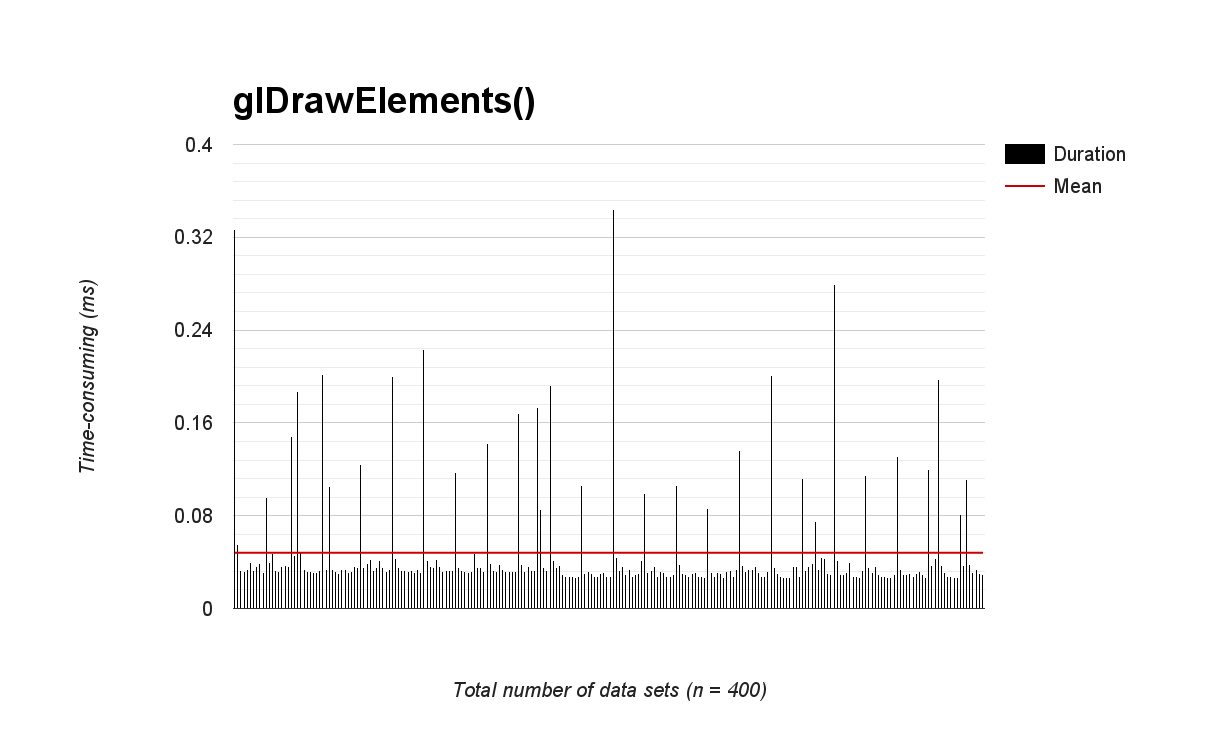
\includegraphics[width=0.9\textwidth, keepaspectratio]{Figures/glDrawElements-performance.png}
	\decoRule
\end{figure}

\begin{figure}[H]
	\caption{glDrawElements performance normal distribution}
	\label{fig:glDrawElements-performance-normal-distribution}
	\centering
	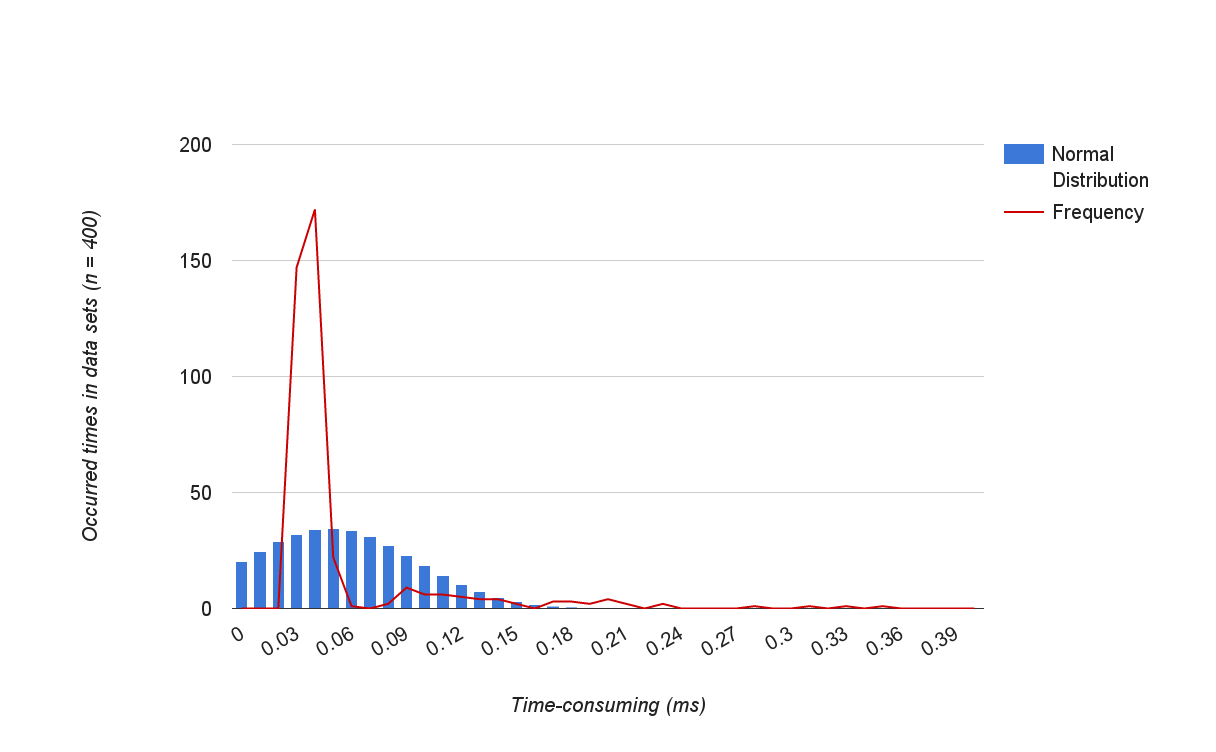
\includegraphics[width=0.9\textwidth, keepaspectratio]{Figures/glDrawElements-performance-normal-distribution.png}
	\decoRule
\end{figure}

This is unacceptable, but the solution is straightforward using one \code{glDrawElements} call for a same kind of models, in particularly \code{Placemark}. Unfortunately, it has not been optimized yet, and it has been postponed to future work due to a limited time. In general, using Interleaved attribute array will do the trick. The optimization also has the great opportunity to improve the duplicated calculation in GPU caused by the current optimization of model update \ref{section:placemarks-update}.

%****************************************************************
